% filepath: main.tex
\documentclass{article}
\usepackage{amsmath} % For math formulas
\usepackage{graphicx} % For including images
\usepackage{hyperref} % For hyperlinks
\usepackage{geometry} % For layout adjustments
\usepackage{listings} % For code blocks
\usepackage{float} % For figure placement
\usepackage{xcolor} % For color

% Set page geometry
\geometry{a4paper, margin=1in}

% Define Python style for listings
\lstdefinestyle{python}{
    language=Python,
    basicstyle=\ttfamily\small,
    keywordstyle=\color{blue},
    commentstyle=\color{green!40!black},
    stringstyle=\color{red},
    showstringspaces=false,
    breaklines=true,
    frame=single,
    numbers=left,
    numberstyle=\tiny\color{gray}
}

\title{Nadaraya-Watson Regression}
\author{Linkang Dong} % Add author if needed
\date{\today}

\begin{document}
\maketitle

\section{Introduction}

This is a simple implementation of the Nadaraya-Watson regression \cite{d2l:attention_pooling,wikipedia:kernel_regression} algorithm in Python.

\section{Data Generation}

We generate some random data from the model:
\[
y = 2\sin(x) + x^{0.8} + \epsilon
\]
where $x$ is uniformly distributed in the range $[0, 5]$ and $\epsilon$ is a Gaussian noise with mean 0 and standard deviation 0.5.

\section{Kernel}

First, we define some kernel functions here, which are used to compute the weights for the Nadaraya-Watson regression. The kernel function $K(\mathbf{d})$ is defined as a function of the distance $\mathbf{d}$ between the query point $\mathbf{q}$ and the training point $\mathbf{k}$. The distance is computed as follows:
\begin{equation*}
    \mathbf{d} = \| \mathbf{q} - \mathbf{k} \|
\end{equation*}

The kernel function is then defined as a function of the distance $\mathbf{d}$, and it can take different forms. The most common ones are:
\begin{align*}
    \text{Gaussian:}& \quad K(\mathbf{d}) = \exp\left(- \frac{\mathbf{d}^2}{2 \sigma^2}\right)
    &&
    \text{Boxcar:} \quad K(\mathbf{d}) = \begin{cases}
        1 & \text{if } \mathbf{d} \leq 1 \\
        0 & \text{otherwise}
    \end{cases} \\     
    \text{Constant:}& \quad K(\mathbf{d}) = 1
    &&
    \text{Epanechikov:} \quad K(\mathbf{d}) = \max\left(0, 1 - \mathbf{d}\right)
\end{align*}

We plot different kernel functions as shown in Figure \ref{fig:kernels}:

\begin{figure}[H]
    \centering
    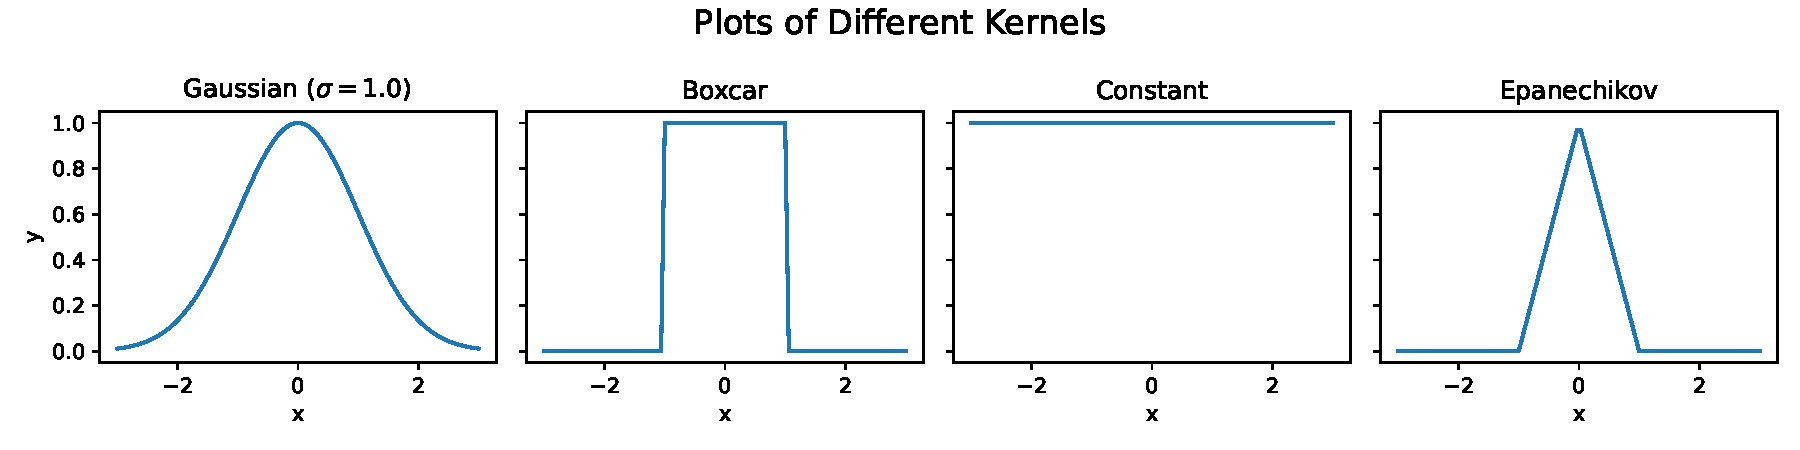
\includegraphics[width=\textwidth]{results/kernels.pdf}
    \caption{Plot of different kernels.}
    \label{fig:kernels}
\end{figure}

Our weights essentially determine the influence of neighboring points on a given point. For the Gaussian kernel, closer points exert a greater influence, while farther points have less impact. With the boxcar kernel, all points within a distance of 1 have equal influence (this distance can be adjusted as a bandwidth parameter), and points beyond this distance have zero influence. The constant kernel assigns equal influence to all points, effectively averaging them. The Epanechnikov kernel resembles a 'hard' Gaussian kernel: influence increases linearly with proximity, but abruptly drops to zero beyond a certain distance.

The Gaussian kernel is the most frequently used. It can be considered a 'soft' version of the boxcar kernel. From a signal processing standpoint, the boxcar kernel acts like a discrete signal, whereas the Gaussian kernel behaves like a continuous signal. In terms of filtering, the boxcar kernel is similar to a band-pass filter (or a low-pass filter if only the positive region is considered), while the Gaussian filter passes all frequencies but attenuates higher frequencies more significantly.

For the Gaussian kernel, the bandwidth can be adjusted by tuning the standard deviation $\sigma$. A larger $\sigma$ results in a wider range of influence from neighboring points, while a smaller $\sigma$ narrows this range. Figure \ref{fig:gaussian_kernels} illustrates Gaussian kernels with varying bandwidths:

\begin{figure}[H]
    \centering
    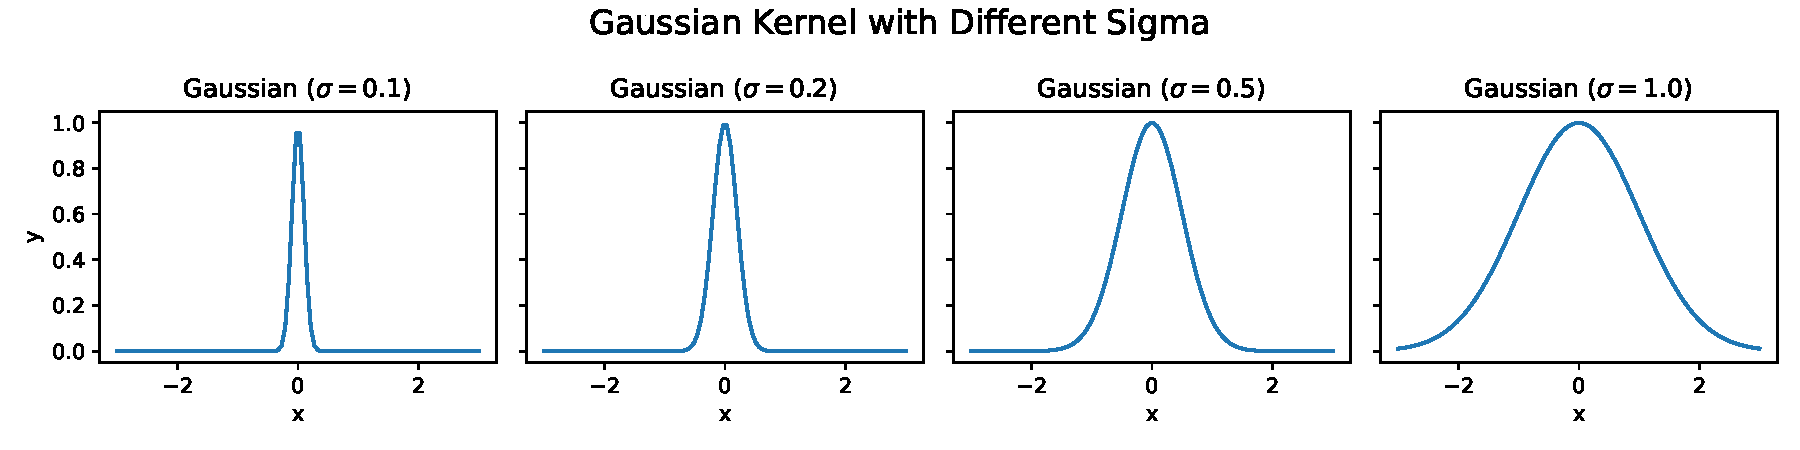
\includegraphics[width=\textwidth]{results/gaussian_kernels.pdf}
    \caption{Gaussian kernel using different bandwidths.}
    \label{fig:gaussian_kernels}
\end{figure}

\section{Nadaraya-Watson Regression}

Our implementation of the Nadaraya-Watson regression algorithm is as follows:

\begin{lstlisting}[style=python]
def nadaraya_watson_regression(x_train, y_train, x_val, kernel):
    diff = x_val.view(-1,1) - x_train.view(1,-1)
    weights = kernel(diff).type(torch.float32)
    weights /= torch.sum(weights, dim=1, keepdim=True)
    y_pred = (weights @ y_train.view(-1,1)).squeeze(1)
    return y_pred
\end{lstlisting}

The few lines of code above essentially encapsulate the core idea of Nadaraya-Watson regression: \textbf{learning by example}. Suppose we have a collected dataset (\texttt{x\_train}, \texttt{y\_train}). We need to use this data to estimate the corresponding values for new data points (\texttt{x\_val}) to predict \texttt{y\_pred}. This utilizes an interpolation-like approach. First, we compute the similarity (or distance, used by the kernel) between the new points \texttt{x\_val} and the training points \texttt{x\_train}. Then, using these similarities as weights (after normalization), we compute a weighted average of the training outputs \texttt{y\_train} to obtain the predicted values \texttt{y\_pred}.

The regression results using different kernel functions are shown in Figure \ref{fig:regression_kernels}. We observe that the Gaussian kernel produces the smoothest result, though it differs somewhat from the true function. The boxcar kernel yields the least smooth result. The constant kernel simply produces a horizontal line (equivalent to averaging all samples). The Epanechnikov kernel gives a result similar to the Gaussian kernel but appears to perform best here.

\begin{figure}[H]
    \centering
    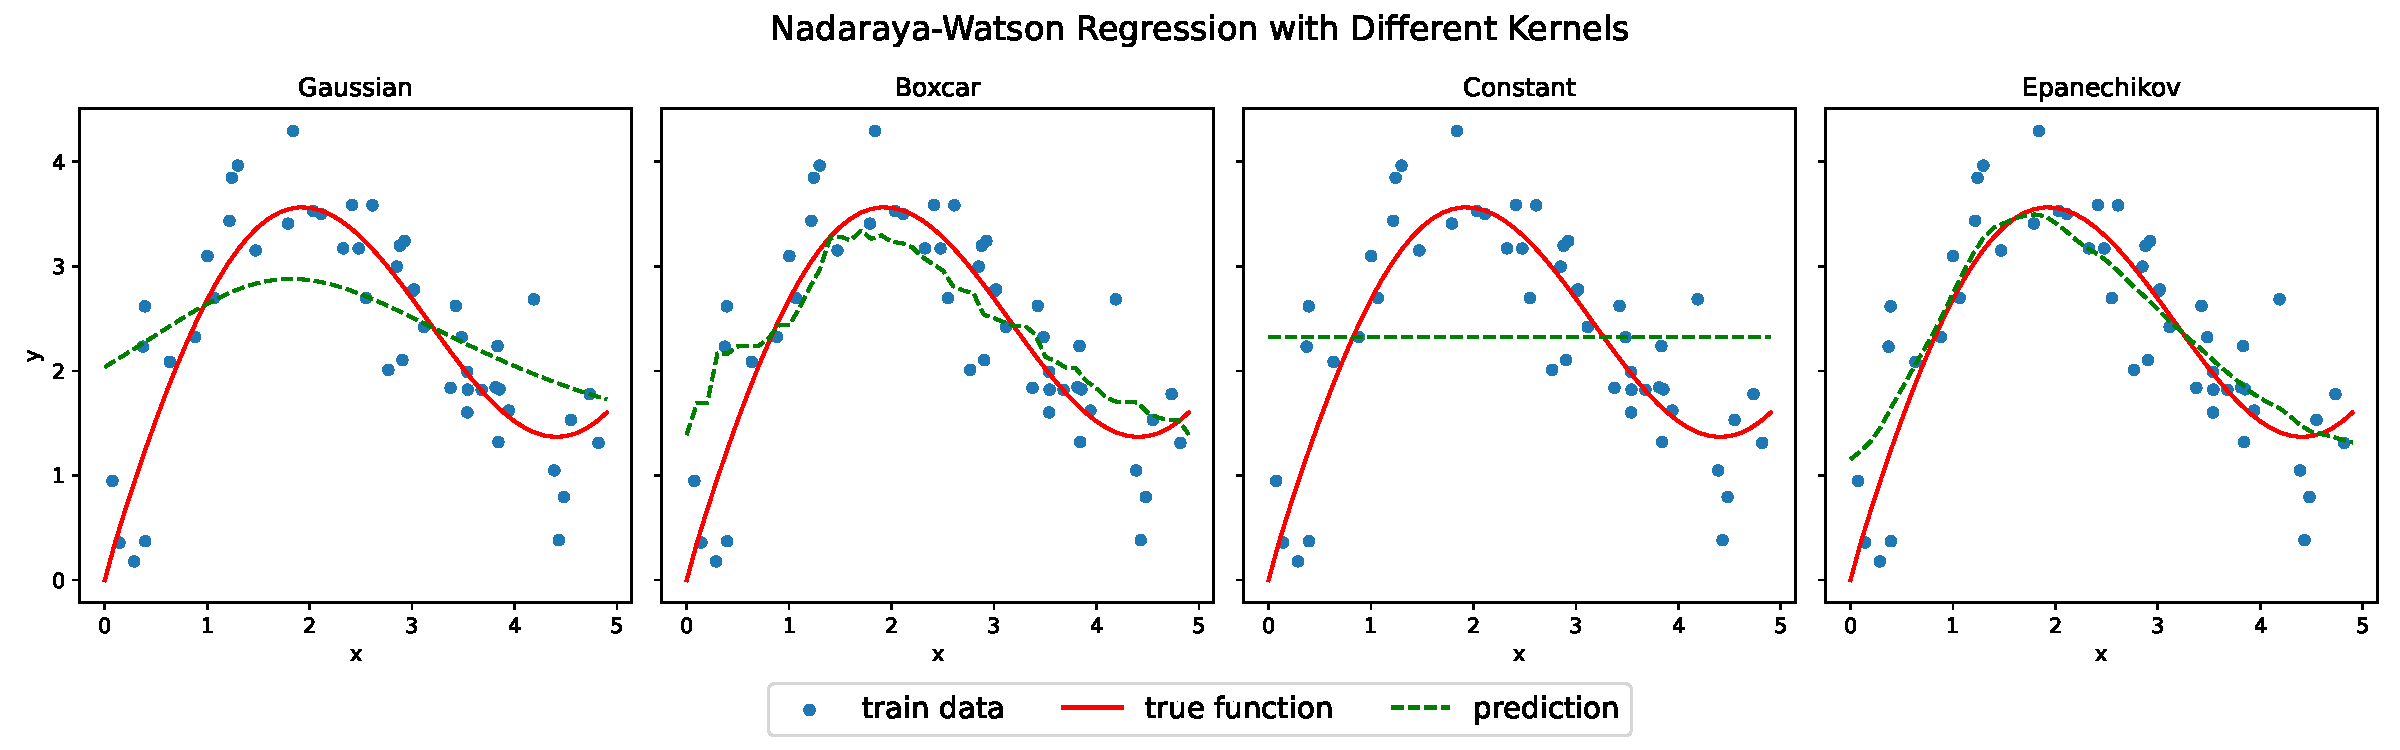
\includegraphics[width=\textwidth]{results/regression_kernels.pdf}
    \caption{Estimated regression function using different kernels.}
    \label{fig:regression_kernels}
\end{figure}

We can also perform regression using different bandwidths. Using the Gaussian kernel, we perform regression with bandwidths of 0.1, 0.2, 0.5, and 1.0, as shown in Figure \ref{fig:adaptive_gaussian}. We observe that a larger bandwidth results in a smoother estimated regression function. At a bandwidth of 0.5, the estimated function is closest to the true function. However, with bandwidths of 0.1 and 0.2, the predicted curve exhibits significant "jittering". This occurs because a very small bandwidth considers only a limited local neighborhood, leading to high variance (similar to overfitting).

\begin{figure}[H]
    \centering
    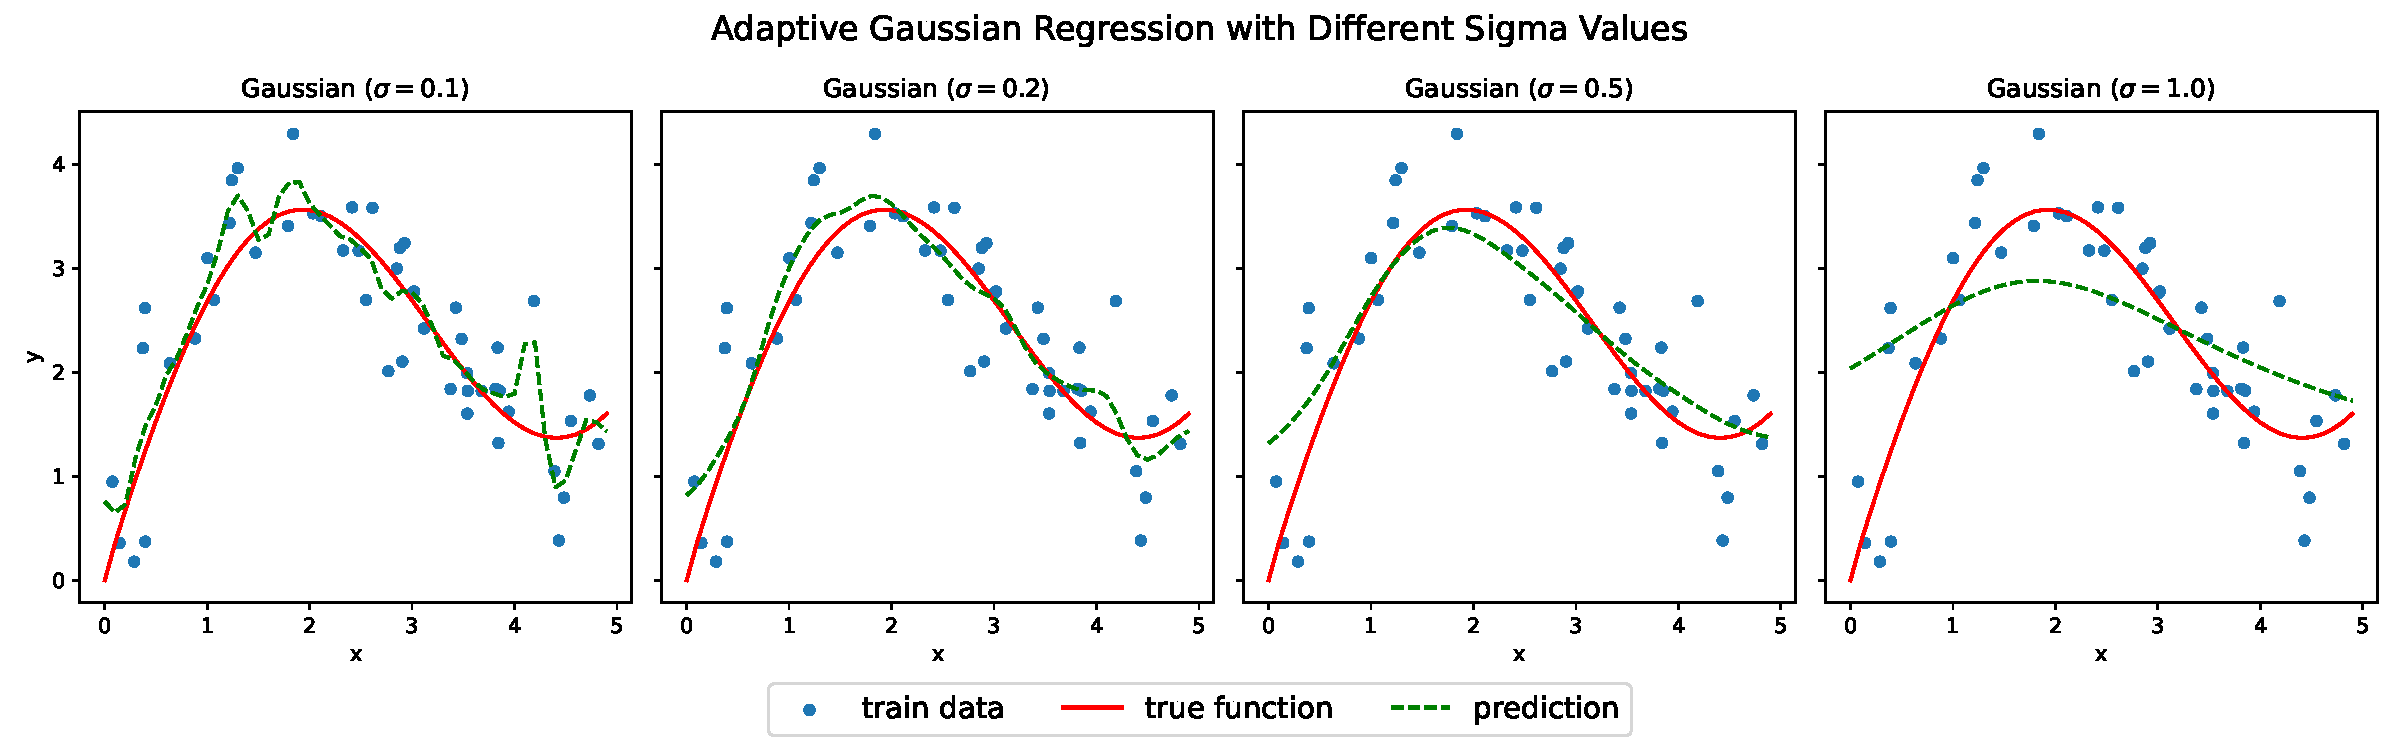
\includegraphics[width=\textwidth]{results/adaptive_gaussian_regression.pdf}
    \caption{Estimated regression function using different bandwidths for the Gaussian kernel.}
    \label{fig:adaptive_gaussian}
\end{figure}

\bibliographystyle{unsrt}
\bibliography{ref}

\end{document}